\providecommand{\Fun}{\operatorname{Fun}}
\providecommand{\QCat}{\mathcal{Q}\mathcal{C}at}
\providecommand{\CSS}{\mathcal{C}\mathcal{S}\mathcal{S}}
\providecommand{\Set}{\mathcal{S}et}
\providecommand{\Cat}{\mathcal{C}at}
\providecommand{\hciso}{\mathbb{I}}  %

\section{带依赖排序的一阶逻辑}\label{sec:first-order-logic-dependent-sorts}

\trInfinityCategory{}论在\trChangeOfModel{}之下的不变性有一项重要的告诫。在从一个%
\trCompleteSegalSpaces{}过渡到其\trUnderlyingQuasiCategory{}再折返之后
\begin{equation*}
\CSS\ \xrightarrow[\ \sim\ ]{\ (-)_{0}\ }\ \QCat\ \xrightarrow[\ \sim\ ]{\ \mathrm{nerve}\ }\ \CSS
\end{equation*}
所得的\trCompleteSegalSpaces{}与原来那个等价，但多半不与之相等。但即便在经典的
严格情形，也并非关于 1-\trCategory{}的每一个陈述都在\trEquivalence{}之下不变：
「此\trCategory{}只有一个对象」就是一个著名的反例。类似地，并非关于 2-\trCategory{}的
每一个陈述都在\trBiequivalence{}之下不变。例如，考虑\cref{prop:cartesian-closure}为诸%
\trHomotopyTwoCategory{}所证明的那个陈述：「此 2-\trCategory{}有一个%
\trTwoTerminalObject」。设 $F\colon\mathcal{C}\Rightarrow\mathcal{D}$ 是 2-\trCategory{}之间的一个%
\trBiequivalence，而 $\mathcal{D}$ 有一个\trTwoTerminalObject{} $t$，那么由本质满性，
存在一个 $s\in\mathcal{C}$ 使得在 $\mathcal{D}$ 中 $Fs\simeq t$。但\trLocalEquivalence{}性质
只提供一支\trEquivalence
\begin{equation*}
\mathcal{C}(c,s)\simeq\mathcal{D}(Fc,Fs)\simeq\mathcal{D}(Fc,t)\cong 1,
\end{equation*}
它使 $s$ 成为一个\emph{双终对象}（biterminal object），却未必是一个%
\trTwoTerminalObject。

模型无关性定理（\cref{thm:biequivalence-of-virtual-equipments}）为由任何一对双等
价的\trInfinityCosmos{}所定义的模的%
\trVirtualEquipment{}提供一个\trBiequivalence。
由于关于\trInfinityCategories{}的重要陈述都可以表述为\trVirtualEquipment{}的性质，
这个\trBiequivalence{}便给出一种机制，使得用∞-\trCategory{}的某一个模型证明的
结果得以借之转移到另一个模型。但是，当一个关于\trInfinityCategories{}的陈述已经以%
\trVirtualEquipment{}的语言表述之后，我们如何能确知它在诸\trVirtualEquipment{}的%
\trBiequivalence{}之下事实上不变呢？

这类问题有一段漫长的历史。Blanc [19] 与 Freyd [43] 刻画了普通\trCategory{}的
那些在\trCategory{}的\trEquivalence{}之下不变的性质（另见 Preller [92]）。Makkai 的
FOLDS 正是为把这些结果推广到诸如 2-\trCategory{}与弱 2-\trCategory{}这样的高阶%
\trCategory{}性结构而发展的 [82]。
在未来的工作中，我们希望对那些在诸\trInfinityCosmos{}的\trBiequivalence{}之下
不变的、关于\trInfinityCategories{}的陈述给出一个完备的刻画\footnote{请注意，我们所
寻求的结果与 Makkai 关于弱 2-\trCategory{}的结果更为接近，而非 Blanc 与 Freyd 关于
1-\trCategory{}的结果；因为我们所关心的是高阶\trCategory{}在换模型之下的不变性，
而不是某个给定模型中诸∞-\trCategory{}之间的\trEquivalence{}之下的不变性。}，但
当前的目标是一个可以说更有用、也远更容易得到的结果。在本节中，我们勾勒 Makkai 的
FOLDS 框架背后的关键想法；下文的全部主要概念与结果都归功于他，尽管我们对定义作了
少许次要的修改，并在记号与术语上有所偏离——这从我们与 Henry [52] 的交谈中汲取了
灵感。在 11.3 节中，我们将应用这一工作来证明：任何能够以\emph{\trVirtualEquipment{}的语言}
——即把 Makkai 的形式语言特殊化到我们在 11.3.2 中引入的一个签名——表述的陈述，
都会给出一个关于\trInfinityCategories{}的模型无关陈述。

Makkai 的 FOLDS 提供了一种形式语言（formal language），用以书写其变量按给定的%
\emph{签名}（signature）组织起来的数学语句。顾名思义，FOLDS 中的语句非常接近
一阶逻辑的语句，只是多了一种重要的新成分。每个变量都被指派属于一个特定的%
\emph{排序}（sort），而这些排序可以依赖于属于更低次数的其他排序的、相容地定义的
变量的有限族。全称量化与存在量化一次只对单一排序的变量定义，而且被量化的公式
不得含有任何依赖于被量化变量的变量。最后，诸如相等之类的关系只容许出现在极大
排序上。例如，在\trCategory{}的语言中，容许写「对所有对象 $x$ 与 $y$、以及所有
从 $x$ 到 $y$ 的箭头 $f$ 与 $g$，$f$ 等于 $g$」，断言该\trCategory{}是一个预序。
但不容许写「存在一个对象 $x$，使得对所有箭头 $h$，$h$ 等于 $1_{x}$」——断言该%
\trCategory{}是终\trCategory{}——因为相等关系遍历的是全部箭头，而非单独一个指定的
hom-集。

在我们引入 FOLDS 语言之前，必须先描述它的签名。

\begin{definition}\label{def:simple-inverse-category}
一个\textbf{简单逆范畴}（simple inverse category）是一个逆范畴（inverse category）
$\mathcal{J}$（见定义 C.1.16），它具有「有限扇出」，意即每个对象仅是有限多支%
箭头的定义域。
这类\trCategory{}的对象可以被赋予典范的次数，只需考察非恒同箭头所成之图：
\begin{itemize}
\item 不是任何（非恒同）箭头之定义域的对象，次数为 $0$；而
\item 其每条（非恒同）「出箭头」的余定义域次数均为 $0$ 的对象被指派次数 $1$；
  如此归纳地继续，
\item 任一对象被指派这样的最小次数：它超过其每条（非恒同）出箭头的余定义域的次数。
\end{itemize}
这定义了一个反射恒同的典范函子 $\mathrm{deg}\colon\mathcal{J}\to\omega^{\mathrm{op}}$。

简单逆\trCategory{}中的一个对象是\textbf{极大的}（maximal），若它不是任何非恒同
箭头的余定义域。
\end{definition}

\begin{definition}\label{def:folds-signature}
一个 \textbf{FOLDS 签名}（FOLDS signature）是一个简单逆\trCategory{}，连同取定的
（可能为空的）一组极大对象，称为「关系符号」（relation symbol）。其余对象则称为
「种类」（kind）。
\end{definition}

FOLDS 签名中的每条非恒同箭头都表示某个种类或关系符号对其他种类的某种依赖，而该%
\trCategory{}中的交换性条件则对这些依赖之间的相容性条件进行编码。下文中，我们以
一点 $\cdot$ 来标示关系符号。

\begin{example}\label{exa:folds-signature-categories}
关于\trCategory{}的 FOLDS 签名 $\mathcal{J}_{\mathcal{C}at}$ 有分别对应于对象与箭头的
两个种类
\begin{center}
\begin{tikzpicture}[x=1.05em,y=1.05em]
  \node (i) at (-7.0,7.5)  {$\dot{I}$};
  \node (T) at (0,8.0)     {$\dot{T}$};
  \node (E) at (7.0,8.0)   {$\dot{E}$};
  \node (A) at (0,0)       {$A$};
  \node (O) at (0,-7.0)    {$O$};
  \draw[->] (-6.2,6.8) -- (-1.2,0.7);
  \node at (-4.4,3.6) {$\scriptstyle i$};
  \draw[->] (-0.35,7.3) -- (-0.35,0.85);
  \draw[->] (0,7.3)    -- (0,0.85);
  \draw[->] (0.35,7.3)  -- (0.35,0.85);
  \node at (-2.3,4.0) {$\scriptstyle \ell\ r\ c$};
  \draw[->] (6.0,7.1) -- (1.5,0.9);
  \draw[->] (7.2,6.9) -- (2.6,0.5);
  \node at (4.6,4.4) {$\scriptstyle \ell$};
  \node at (3.4,2.9) {$\scriptstyle r$};
  \draw[->] (-0.7,-0.85) -- (-0.7,-6.1);
  \draw[->] (0.7,-0.85)  -- (0.7,-6.1);
  \node at (-0.35,-3.5) {$\scriptstyle s$};
  \node at (0.35,-3.5)  {$\scriptstyle t$};
\end{tikzpicture}
\end{center}
连同复合关系
\begin{equation*}
\begin{array}{ccc}
s\cdot i = t\cdot i & s\cdot c = s\cdot \ell & s\cdot \ell = s\cdot r\\
 & t\cdot c = t\cdot r & t\cdot \ell = t\cdot r\\
 & t\cdot \ell = s\cdot r &
\end{array}
\end{equation*}
在此例中，每个极大对象都是一个关系符号。一元关系符号 $\dot{I}$ 编码恒同箭头，
$\dot{T}$ 见证三元复合关系，而 $\dot{E}$ 则表达平行箭头的相等。
\end{example}

\begin{example}\label{exa:folds-signature-2-categories}
关于 2-\trCategory{}的 FOLDS 签名 $\mathcal{J}_{2\text{-}\mathcal{C}at}$ 有对应于 0-、1-与
2-\trCell{}的种类，还有对应于恒同 1-\trCell{}与 1-\trCell{}之复合的种类。此外尚有关于
平行 2-\trCell{}之相等、恒同 2-\trCell{}、以及 2-\trCell{}的竖直复合与水平复合的关系
符号：
\begin{center}
\begin{tikzpicture}[x=1.05em,y=1.05em]
  \node (V) at (0,11.5)    {$\dot{V}$};
  \node (E) at (7.5,11.5)  {$\dot{E}$};
  \node (H) at (-7.5,6.5)  {$\dot{H}$};
  \node (C2) at (0,6.5)    {$C_{2}$};
  \node (I2) at (7.0,6.5)  {$\dot{I}_{2}$};
  \node (T) at (-7.5,1.0)  {$T$};
  \node (C1) at (0,1.0)    {$C_{1}$};
  \node (I1) at (7.0,1.0)  {$I_{1}$};
  \node (C0) at (0,-4.5)   {$C_{0}$};
  \draw[->] (-0.35,10.8) -- (-0.35,7.4);
  \draw[->] (0,10.8)     -- (0,7.4);
  \draw[->] (0.35,10.8)  -- (0.35,7.4);
  \node at (-2.4,9.1) {$\scriptstyle \ell\ r\ c$};
  \draw[->] (6.7,10.6) -- (2.0,7.2);
  \draw[->] (7.9,10.4) -- (3.0,6.8);
  \node at (5.3,9.0)  {$\scriptstyle \ell$};
  \node at (4.1,7.6)  {$\scriptstyle r$};
  \draw[->] (6.0,6.5) -- (1.4,6.5);
  \node at (3.7,6.95) {$\scriptstyle i$};
  \draw[->] (-6.3,6.9) -- (-1.4,6.9);
  \draw[->] (-6.3,6.5) -- (-1.4,6.5);
  \draw[->] (-6.3,6.1) -- (-1.4,6.1);
  \node at (-3.9,7.25) {$\scriptstyle c$};
  \node at (-3.9,6.7)  {$\scriptstyle r$};
  \node at (-3.9,6.3)  {$\scriptstyle \ell$};
  \draw[->] (-7.85,5.8) -- (-7.85,1.7);
  \draw[->] (-7.15,5.8) -- (-7.15,1.7);
  \node at (-7.72,3.75) {$\scriptstyle s$};
  \node at (-7.28,3.75) {$\scriptstyle t$};
  \draw[->] (-6.3,1.4) -- (-1.4,1.4);
  \draw[->] (-6.3,1.0) -- (-1.4,1.0);
  \draw[->] (-6.3,0.6) -- (-1.4,0.6);
  \node at (-3.9,1.75) {$\scriptstyle c$};
  \node at (-3.9,1.2)  {$\scriptstyle r$};
  \node at (-3.9,0.8)  {$\scriptstyle \ell$};
  \draw[->] (6.0,1.0) -- (1.4,1.0);
  \node at (3.7,1.45) {$\scriptstyle i$};
  \draw[->] (-0.35,5.8) -- (-0.35,1.7);
  \draw[->] (0.35,5.8)  -- (0.35,1.7);
  \node at (-0.28,3.75) {$\scriptstyle s$};
  \node at (0.28,3.75)  {$\scriptstyle t$};
  \draw[->] (-0.35,0.3) -- (-0.35,-3.8);
  \draw[->] (0.35,0.3)  -- (0.35,-3.8);
  \node at (-0.28,-1.75) {$\scriptstyle s$};
  \node at (0.28,-1.75)  {$\scriptstyle t$};
\end{tikzpicture}
\end{center}
逆范畴 $\mathcal{J}_{2\text{-}\mathcal{C}at}$ 具有来自底 1-\trCategory{}的关系
\begin{equation*}
s\cdot i = t\cdot i\qquad s\cdot c = s\cdot \ell\qquad t\cdot c = t\cdot r\qquad t\cdot \ell = s\cdot r,
\end{equation*}
球状性关系
\begin{equation*}
s\cdot s = s\cdot t\qquad\qquad t\cdot s = t\cdot t,
\end{equation*}
支配竖直复合、恒同、以及平行 2-\trCell{}之间的相等的关系
\begin{equation*}
\begin{array}{ccc}
s\cdot i = t\cdot i & s\cdot c = s\cdot \ell & s\cdot \ell = s\cdot r\\
 & t\cdot c = t\cdot r & t\cdot \ell = t\cdot r\\
 & t\cdot \ell = s\cdot r &
\end{array}
\end{equation*}
再加上把水平复合与 1-\trCell{}的复合联系起来的关系
\begin{equation*}
\begin{array}{ccc}
s\cdot \ell = \ell\cdot s & s\cdot r = r\cdot s & s\cdot c = c\cdot s\\
t\cdot \ell = \ell\cdot t & t\cdot r = r\cdot t & t\cdot c = c\cdot t.
\end{array}
\end{equation*}
\end{example}

\begin{definition}\label{def:j-structure}
对于一个给定的 FOLDS 签名 $\mathcal{J}$，一个 \textbf{$\mathcal{J}$-结构}
（$\mathcal{J}$-structure）是一个\trFunctor{} $M\colon\mathcal{J}\to\Set$，使得对每个
关系符号 $\dot{R}\in\mathcal{J}$，由定义域为 $\dot{R}$ 的那族非恒同箭头所诱导的映射
\begin{equation*}
M\dot{R}\longrightarrow\prod_{p\colon \dot{R}\to^{\neq}K_{p}} MK_{p}
\end{equation*}
是一个\trMonomorphism。\footnote{陈述这一条件的另一种——可以说更有用的——方式，
是要求\cref{obs:matching-maps}的那些匹配映射在诸关系符号处的分量都是%
\trMonomorphism{}（见\cref{ex:folds-matching-map-mono}）。}
\end{definition}

\begin{example}\label{exa:d-cat-nerve}
考虑\trFunctor{} $D_{\mathcal{C}at}\colon\mathcal{J}_{\mathcal{C}at}^{\mathrm{op}}\to\Cat$，其像由下图给出
\begin{center}
\begin{tikzpicture}[x=1.05em,y=1.05em]
  \node (IT) at (-6.5,4.2) {$1$};
  \node (T)  at (0,4.6)    {$3$};
  \node (E)  at (6.0,4.6)  {$2$};
  \node (A)  at (0,0)      {$2$};
  \node (O)  at (0,-4.2)   {$1$};
  \draw[->] (-1.3,0.75) -- (-1.3,3.95);
  \draw[->] (0,0.75)    -- (0,3.95);
  \draw[->] (1.3,0.75)  -- (1.3,3.95);
  \node at (-2.05,2.4) {$\scriptstyle\delta^{2}$};
  \node at (-0.55,2.4) {$\scriptstyle\delta^{0}$};
  \node at (2.0,2.4)   {$\scriptstyle\delta^{1}$};
  \draw[->] (-1.4,0.55) -- (-5.7,4.0);
  \node at (-4.2,2.7) {$\scriptstyle !$};
  \draw[->] (1.5,0.65) -- (5.3,4.3);
  \draw[->] (2.2,0.5)  -- (6.3,4.0);
  \node at (3.6,3.0) {$\scriptstyle \mathrm{id}$};
  \node at (4.9,2.3) {$\scriptstyle \mathrm{id}$};
  \draw[->] (-0.7,-3.4) -- (-0.7,-0.75);
  \draw[->] (0.7,-3.4)  -- (0.7,-0.75);
  \node at (-1.35,-2.1) {$\scriptstyle 0$};
  \node at (1.35,-2.1)  {$\scriptstyle 1$};
\end{tikzpicture}
\end{center}
从 $D_{\mathcal{C}at}$ 映出便定义了一个\trFunctor{}
$M_{-}\colon\Cat\to\Set^{\mathcal{J}_{\mathcal{C}at}}$，其像位于 $\mathcal{J}_{\mathcal{C}at}$-结构的满子%
\trCategory{}之中。\footnote{这之所以成立，是因为图表 $D_{\mathcal{C}at}$ 在对象 $\dot{I}$、%
$\dot{T}$ 与 $\dot{E}$ 处的\trLatchingMap{}（latching maps，见定义 C.4.14）各自定义一个%
\trEpimorphism{}——即\trCategory{}之间的满射\trFunctor。}
对任何小 1-\trCategory{} $C$，$M_{C}O$ 就是对象之集，$M_{C}A$ 就是箭头之集，而
$M_{C}\dot{I}$、$M_{C}\dot{T}$ 与 $M_{C}\dot{E}$ 则分别编码检测恒同箭头、交换三角形、
以及平行箭头之相等的关系。
\end{example}

\begin{example}\label{exa:e-d-functors-2cat}
考虑诸\trFunctor{} $E_{2\text{-}\mathcal{C}at}$ 与
$D_{2\text{-}\mathcal{C}at}\colon\mathcal{J}_{2\text{-}\mathcal{C}at}^{\mathrm{op}}\to 2\text{-}\Cat$\footnote{原书函子域印作
$\mathcal{J}_{2\text{-}\mathcal{C}at}$，疑漏上标 ${}^{\mathrm{op}}$：\cref{exa:d-cat-nerve}之同款函子域作
$\mathcal{J}_{\mathcal{C}at}^{\mathrm{op}}$，\cref{lem:surjective-equivalence-fiberwise-surjection}证明中 hom-二函子
之域亦作 $(2\text{-}\Cat^{\mathcal{J}_{2\text{-}\mathcal{C}at}^{\mathrm{op}}})^{\mathrm{op}}$，此处径补。——译者注}，定义如下
\begin{center}
\begin{tikzpicture}[x=1.05em,y=1.05em]
  \node (S3) at (1.0,7.0)   {$\Sigma[3]$};
  \node (S2t) at (6.0,8.0)  {$\Sigma[2]$};
  \node (Ed) at (-6.5,3.0)  {$\mathbb{H}_{=}$};
  \node (S2) at (1.0,3.0)   {$\Sigma[2]$};
  \node (tw) at (6.0,3.0)   {$2$};
  \node (tr) at (-6.5,-1.5) {$3$};
  \node (tc) at (1.0,-1.5)  {$2$};
  \node (on) at (6.0,-1.5)  {$1$};
  \node (ob) at (1.0,-6.0)  {$1$};
  \draw[->] (0.3,3.75) -- (0.3,6.3);
  \draw[->] (1.0,3.75) -- (1.0,6.3);
  \draw[->] (1.7,3.75) -- (1.7,6.3);
  \draw[->] (2.3,3.7) -- (5.1,7.3);
  \draw[->] (3.0,3.6) -- (5.8,7.6);
  \draw[->] (-2.6,3.3) -- (-5.3,3.3);
  \draw[->] (-2.6,3.0) -- (-5.3,3.0);
  \draw[->] (-2.6,2.7) -- (-5.3,2.7);
  \draw[->] (2.6,3.0) -- (4.6,3.0);
  \draw[->] (-6.8,-0.75) -- (-6.8,2.2);
  \draw[->] (-6.2,-0.75) -- (-6.2,2.2);
  \draw[->] (-2.6,-1.8) -- (-5.3,-1.8);
  \draw[->] (-2.6,-1.5) -- (-5.3,-1.5);
  \draw[->] (-2.6,-1.2) -- (-5.3,-1.2);
  \draw[->] (0.4,-0.75) -- (0.4,2.2);
  \draw[->] (1.6,-0.75) -- (1.6,2.2);
  \draw[->] (2.6,-1.5) -- (4.6,-1.5);
  \draw[->] (0.3,-5.25) -- (0.3,-2.25);
  \draw[->] (1.7,-5.25) -- (1.7,-2.25);
\end{tikzpicture}
\qquad
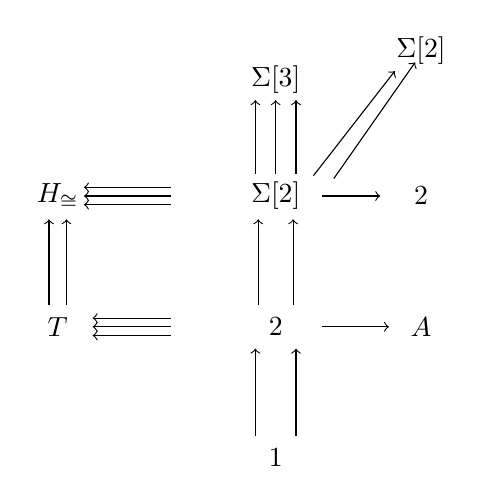
\begin{tikzpicture}[x=1.05em,y=1.05em]
  \node (S3) at (1.0,7.0)   {$\Sigma[3]$};
  \node (S2t) at (6.0,8.0)  {$\Sigma[2]$};
  \node (Ed) at (-6.5,3.0)  {$\mathbb{H}_{\cong}$};
  \node (S2) at (1.0,3.0)   {$\Sigma[2]$};
  \node (tw) at (6.0,3.0)   {$2$};
  \node (tr) at (-6.5,-1.5) {$\mathbb{T}$};
  \node (tc) at (1.0,-1.5)  {$2$};
  \node (on) at (6.0,-1.5)  {$\mathbb{A}$};
  \node (ob) at (1.0,-6.0)  {$1$};
  \draw[->] (0.3,3.75) -- (0.3,6.3);
  \draw[->] (1.0,3.75) -- (1.0,6.3);
  \draw[->] (1.7,3.75) -- (1.7,6.3);
  \draw[->] (2.3,3.7) -- (5.1,7.3);
  \draw[->] (3.0,3.6) -- (5.8,7.6);
  \draw[->] (-2.6,3.3) -- (-5.6,3.3);
  \draw[->] (-2.6,3.0) -- (-5.6,3.0);
  \draw[->] (-2.6,2.7) -- (-5.6,2.7);
  \draw[->] (2.6,3.0) -- (4.6,3.0);
  \draw[->] (-6.8,-0.75) -- (-6.8,2.2);
  \draw[->] (-6.2,-0.75) -- (-6.2,2.2);
  \draw[->] (-2.6,-1.8) -- (-5.3,-1.8);
  \draw[->] (-2.6,-1.5) -- (-5.3,-1.5);
  \draw[->] (-2.6,-1.2) -- (-5.3,-1.2);
  \draw[->] (0.4,-0.75) -- (0.4,2.2);
  \draw[->] (1.6,-0.75) -- (1.6,2.2);
  \draw[->] (2.6,-1.5) -- (4.9,-1.5);
  \draw[->] (0.3,-5.25) -- (0.3,-2.25);
  \draw[->] (1.7,-5.25) -- (1.7,-2.25);
\end{tikzpicture}
\end{center}
其中
\begin{center}
\begin{tikzpicture}[x=1.05em,y=1.05em]
  \node at (-9.5,0.4) {$\mathbb{T}\coloneqq$};
  \node (a) at (-4.5,1.4) {$\bullet$};
  \node (b) at (-6.5,-1.2) {$\bullet$};
  \node (c) at (-2.0,-1.2) {$\bullet$};
  \draw[->] (-5.0,0.8) -- (-6.1,-0.6);
  \draw[->] (-4.0,0.8) -- (-2.6,-0.6);
  \node at (-5.9,0.1) {$\scriptstyle\cong$};
  \draw[->] (-5.9,-1.2) -- (-2.7,-1.2);
  \node at (-0.9,0.4) {，};
  \node at (0.4,0.4) {$\mathbb{A}\coloneqq$};
  \node (d) at (3.2,0.1) {$\bullet$};
  \draw[->] (3.2,0.75) arc[start angle=110,end angle=430,radius=0.62];
  \node at (4.6,0.75) {$\scriptstyle\cong$};
  \node at (5.6,0.4) {，$\Sigma2\coloneqq$};
  \node (e) at (9.0,0.1) {$\bullet$};
  \node (f) at (12.2,0.1) {$\bullet$};
  \draw[->] (9.4,0.45) to[bend left=18] (11.8,0.45);
  \draw[->] (9.4,-0.25) to[bend right=18] (11.8,-0.25);
  \node at (10.6,0.35) {$\scriptstyle\Downarrow$};
  \node at (13.3,0.4) {，$\Sigma[3]\coloneqq$};
  \node (g) at (17.4,0.1) {$\bullet$};
  \node (h) at (20.6,0.1) {$\bullet$};
  \draw[->] (17.8,0.45) to[bend left=18] (20.2,0.45);
  \draw[->] (17.8,-0.25) to[bend right=18] (20.2,-0.25);
  \node at (19.0,0.55) {$\scriptstyle\Downarrow$};
  \node at (19.0,-0.45) {$\scriptstyle\Downarrow$};
  \node at (21.6,0.4) {，};
\end{tikzpicture}
\end{center}
\begin{center}
\begin{tikzpicture}[x=1.05em,y=1.05em]
  \node at (-7.2,0.4) {$\mathbb{H}_{=}\coloneqq$};
  \node (a) at (-3.4,0.1) {$\bullet$};
  \node (b) at (-0.6,0.1) {$\bullet$};
  \node (c) at (2.2,0.1) {$\bullet$};
  \draw[->] (-3.0,0.45) to[bend left=18] (-1.0,0.45);
  \draw[->] (-3.0,-0.25) to[bend right=18] (-1.0,-0.25);
  \node at (-2.0,0.35) {$\scriptstyle\Downarrow$};
  \draw[->] (-0.2,0.45) to[bend left=18] (1.8,0.45);
  \draw[->] (-0.2,-0.25) to[bend right=18] (1.8,-0.25);
  \node at (0.8,0.35) {$\scriptstyle\Downarrow$};
  \node at (3.3,0.4) {，};
  \node at (4.6,0.4) {以及};
  \node at (7.4,0.4) {$\mathbb{H}_{\cong}\coloneqq$};
  \node (d) at (10.6,0.1) {$\bullet$};
  \node (e) at (13.4,0.1) {$\bullet$};
  \node (f) at (16.2,0.1) {$\bullet$};
  \draw[->] (11.0,0.45) to[bend left=18] (13.0,0.45);
  \draw[->] (11.0,-0.25) to[bend right=18] (13.0,-0.25);
  \node at (12.0,0.35) {$\scriptstyle\Downarrow$};
  \draw[->] (13.8,0.45) to[bend left=18] (15.8,0.45);
  \draw[->] (13.8,-0.25) to[bend right=18] (15.8,-0.25);
  \node at (14.8,0.35) {$\scriptstyle\Downarrow$};
  \draw[->] (11.0,0.9) to[bend left=38] (15.8,0.9);
  \node at (13.4,2.5) {$\scriptstyle\cong$};
  \draw[->] (11.0,-0.7) to[bend right=38] (15.8,-0.7);
  \node at (13.4,-2.4) {$\scriptstyle\cong$};
\end{tikzpicture}
\end{center}
它们都是由所描绘的数据生成的自由 2-\trCategory。图表 $D_{2\text{-}\mathcal{C}at}$ 可以
理解为 $E_{2\text{-}\mathcal{C}at}$ 相对于 Lack 的 2-\trCategory{}模型结构（见定理
C.5.14）的一个 Reedy 余纤维性替换，在该模型结构中，余纤维化是那些在对象与
1-\trCell{}上均为单射的 2-\trFunctor，而平凡纤维化则是满射等价 [71]。
\end{example}

从 $E_{2\text{-}\mathcal{C}at}$ 或从 $D_{2\text{-}\mathcal{C}at}$ 映出便定义诸\trFunctor
$N_{-}$ 与 $M_{-}\colon 2\text{-}\Cat\to\Set^{\mathcal{J}_{2\text{-}\mathcal{C}at}}$，其像位于
$\mathcal{J}_{2\text{-}\mathcal{C}at}$-结构的满子\trCategory{}之中。\footnote{同样地，各
图表在全部四个关系符号处的\trLatchingMap{}都是\trEpimorphism。}我们把 $M_{\mathcal{C}}$ 称为
配属于一个 2-\trCategory{} $\mathcal{C}$ 的「饱和」$\mathcal{J}_{2\text{-}\mathcal{C}at}$-结构，
而把 $N_{\mathcal{C}}$ 称为「朴素」$\mathcal{J}_{2\text{-}\mathcal{C}at}$-结构。

\begin{observation}[匹配映射的纤维]\label{obs:matching-maps}
对每个 $\mathcal{J}$-结构 $M\colon\mathcal{J}\to\Set$ 与对象 $K\in\mathcal{J}$——无论
其为一个种类还是一个关系符号——都存在一个典范的\textbf{匹配映射}（matching map）
\begin{center}
\begin{tikzpicture}[x=1.05em,y=1.05em]
  \node (MK) at (0,0.9) {$MK$};
  \node (prod) at (9.5,0.9)
    {$\displaystyle\prod_{p\colon K\to^{\neq}K_{p}} MK_{p}$};
  \node (lim) at (4.2,-1.3)
    {$\partial^{K}M\coloneqq\displaystyle\lim_{p\colon K\to^{\neq}K_{p}} MK_{p}$};
  \draw[->] (1.3,0.9) -- (6.6,0.9);
  \draw[->,dashed] (0.5,0.3) -- (2.9,-0.7);
  \node at (0.9,-0.55) {$\scriptstyle m^{K}$};
  \draw[right hook->] (6.0,-0.9) -- (8.3,0.35);
\end{tikzpicture}
\end{center}
其余定义域是观察 C.1.18 所定义的匹配对象。注意，极限与积都取遍以 $K$ 为定义域的
非恒同箭头——这一隐含条件也适用于下文的类似构造。我们把一个 $\mathcal{J}$-结构
$M$ 设想为一种结构化的集合：其中每个集合 $MK$ 都被进一步分割为匹配映射
$m^{K}\colon MK\to\partial^{K}M$ 的诸\trFiber。
\end{observation}

现在我们来描述 Makkai 的「依赖排序」——它们与其变量一道经由相互递归得到定义。
这些变量可以纯粹以句法方式引入，但我们发现更直观的做法是把它们设想为属于一个%
\textbf{上下文}（context）：此即一个 $\mathcal{J}$-结构 $\Gamma$，其中与每个种类
$K\in\mathcal{J}$ 相关联的集合 $\Gamma K$ 两两不交。

\begin{definition}[排序及其变量]\label{def:sorts-variables}
取定一个 FOLDS 签名 $\mathcal{J}$ 与一个上下文 $\Gamma\colon\mathcal{J}\to\Set$。
\begin{itemize}
\item 每个次数为零的种类 $K$ 都定义一个\textbf{排序}，亦记作 $K$，其变量就是集合
  $\Gamma K$ 的元素。书写「$x:K$」意谓 $x\in\Gamma K$，即 $x$ 是属于上下文 $\Gamma$
  中排序 $K$ 的一个变量。
\item 对每个次数为一的种类 $K$，匹配映射 $m^{K}$ 取下示之形，其中积取遍
  $\mathcal{J}$ 中以 $K$ 为定义域、余定义域次数为零的那些箭头。对任何变量族
  $\{x_{p}\mathbin{:}K_{p}\}_{p\colon K\to^{\neq}K_{p}}$，就有排序 $K\langle x_{p}\rangle$：
  其变量是纤维
\begin{center}
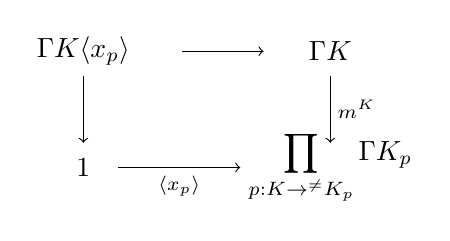
\begin{tikzpicture}[x=1.05em,y=1.05em]
  \node (tl) at (0,3)   {$\Gamma K\langle x_{p}\rangle$};
  \node (tr) at (8.5,3) {$\Gamma K$};
  \node (bl) at (0,-1)  {$1$};
  \node (br) at (8.5,-1)
    {$\displaystyle\prod_{p\colon K\to^{\neq}K_{p}}\Gamma K_{p}$};
  \draw[->] (3.4,3) -- (6.2,3);
  \draw[->] (0,2.15) -- (0,-0.15);
  \draw[->] (8.5,2.15) -- (8.5,-0.15);
  \node at (9.4,1.0) {$\scriptstyle m^{K}$};
  \draw[->] (1.2,-1) -- (5.4,-1);
  \node at (3.3,-1.65) {$\scriptstyle\langle x_{p}\rangle$};
  \node at (1.05,2.45) {$\scriptstyle\lrcorner$};
\end{tikzpicture}
\end{center}
  的元素，并且称这些变量\textbf{依赖}于诸变量 $x_{p}:K_{p}$。
\item 对次数更高的种类 $K$，变量族
  $\{x_{p}\mathbin{:}K_{p}(x_{q_{p}})\}_{p\colon K\to^{\neq}K_{p}}$
  是\textbf{相容的}，若 $(x_{p})\in\prod_{p\colon K\to^{\neq}K_{p}}\Gamma K_{p}$ 属于匹配
  对象 $\partial^{K}\Gamma$。在实践中，这意味着列表中较高次的变量按 FOLDS 签名中
  依赖关系所规定的方式依赖于较低次的变量。对任何相容的变量族，都有排序
  $K\langle x_{p}\rangle$：其变量是匹配映射 $m^{K}$ 在
  $\langle x_{p}\rangle\in\partial^{K}\Gamma$ 之上的\trFiber{}的元素
\begin{center}
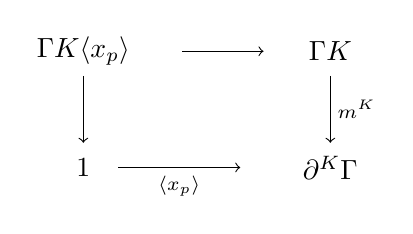
\begin{tikzpicture}[x=1.05em,y=1.05em]
  \node (tl) at (0,3)   {$\Gamma K\langle x_{p}\rangle$};
  \node (tr) at (8.5,3) {$\Gamma K$};
  \node (bl) at (0,-1)  {$1$};
  \node (br) at (8.5,-1) {$\partial^{K}\Gamma$};
  \draw[->] (3.4,3) -- (6.2,3);
  \draw[->] (0,2.15) -- (0,-0.15);
  \draw[->] (8.5,2.15) -- (8.5,-0.15);
  \node at (9.4,1.0) {$\scriptstyle m^{K}$};
  \draw[->] (1.2,-1) -- (5.4,-1);
  \node at (3.3,-1.65) {$\scriptstyle\langle x_{p}\rangle$};
  \node at (1.05,2.45) {$\scriptstyle\lrcorner$};
\end{tikzpicture}
\end{center}
\end{itemize}

按照约定，在排序的规约中显式列出的变量只有最高次的那些变量；这些变量所依赖的
较低次变量，则可从最高次变量所属的排序推得。
\end{definition}

\begin{example}\label{exa:sorts-jcat}
对 FOLDS 签名 $\mathcal{J}_{\mathcal{C}at}$ 而言：
\begin{itemize}
\item 有一个排序 $O$。
\item 对任何一对变量 $x$ 与 $y:O$，有一个排序 $A(x,y)$。
\end{itemize}
\end{example}

\begin{example}\label{exa:sorts-j2cat}
对 FOLDS 签名 $\mathcal{J}_{2\text{-}\mathcal{C}at}$ 而言：
\begin{itemize}
\item 有一个排序 $C_{0}$。
\item 对任何一对变量 $x$ 与 $y:C_{0}$，有一个排序 $C_{1}(x,y)$。
\item 对任何 $x$ 与 $y:C_{0}$、以及 $f$ 与 $g:C_{1}(x,y)$，有一个排序
  $C_{2}(x,y,f,g)$。这个排序通常缩写作 $C_{2}\langle f,g\rangle$，其隐含变量
  $x$ 与 $y:C_{0}$ 可由变量 $f$ 与 $g$ 所居住的排序推知。
\end{itemize}
\end{example}

沿用同样的缩写：
\begin{itemize}
\item 对任何 $x:C_{0}$ 与 $f:C_{1}(x,x)$，有一个排序 $I_{1}(f)$。
\item 对任何 $x$、$y$、$z:C_{0}$ 以及 $f:C_{1}(x,y)$、$g:C_{1}(y,z)$ 与
  $h:C_{1}(x,z)$，有一个排序 $T\langle f,g,h\rangle$。
\end{itemize}

我们现在已准备好引入与一个 FOLDS 签名 $\mathcal{J}$ 相关联的形式语言的公式与语句。
它们由递归定义，从原子公式出发，而原子公式由诸关系符号支配。再次取定一个 FOLDS
签名 $\mathcal{J}$ 与一个上下文 $\Gamma\colon\mathcal{J}\to\Set$。

\begin{definition}\label{def:atomic-formula}
带依赖排序的逻辑中的一个\textbf{原子公式}（atomic formula）是形如
$\dot{R}\langle x_{p}\rangle$ 的一个实体，其中 $\dot{R}$ 是一个关系符号，而变量
$\{x_{p}\mathbin{:}K_{p}(x_{q_{p}})\}_{p\colon \dot{R}\to^{\neq}K_{p}}$
必须定义一个相容族，意即它们定义了一个元素
$\langle x_{p}\rangle\in\partial^{\dot{R}}\Gamma$。
\end{definition}

\begin{example}\label{exa:atomic-formula-commutative-triangle}
在 FOLDS 签名 $\mathcal{J}_{\mathcal{C}at}$ 中，对任何 $x$、$y$、$z:O$ 以及
$f:A(x,y)$、$g:A(y,z)$ 与 $h:A(x,z)$，都有一个原子公式
$\dot{T}\langle x,y,z,f,g,h\rangle$，缩写作 $\dot{T}\langle f,g,h\rangle$，它可以被
设想为断言由箭头 $f$、$g$ 与 $h$ 构成的三角形的交换性。
\end{example}

\begin{digression}\label{dig:restricted-equality}
FOLDS 哲学的一个关键想法是：它应当表达一种带受限相等性的逻辑。这一点在 FOLDS
签名 $\mathcal{J}_{\mathcal{C}at}$ 与 $\mathcal{J}_{2\text{-}\mathcal{C}at}$ 中清晰可见：
二者在种类 $A$ 与 $C_{2}$ 上包含二元相等关系符号，但在这些种类所依赖的种类
$O$、$C_{0}$ 与 $C_{1}$ 上却不配备类似的相等谓词。更精确地说，$\mathcal{J}_{\mathcal{C}at}$
的原子公式 $\dot{E}(f,g)$ 与 $\mathcal{J}_{2\text{-}\mathcal{C}at}$ 的原子公式
$\dot{E}(\alpha,\beta)$ 可用于表达一对平行箭头的相等，因为相容性要求对某对
$x$ 与 $y:O$ 有 $f$ 与 $g:A(x,y)$；亦可用于表达平行 2-\trCell{}的相等，因为相容性
要求对某对 $f$ 与 $g:C_{1}(x,y)$ 及某对 $x$ 与 $y:C_{0}$\footnote{原书此两处分别
印作「$\alpha,\beta:C_{1}\langle f,g\rangle$」与「$x,y:O$」（2026-09-15 机械
波次经 booktext 文本层复核证实，唯原引录括号有误，径正）。按例 11.2.11 所立
之排序口径，平行 2-\trCell{}居于排序 $C_{2}\langle f,g\rangle$ 之中，且
$C_{1}(x,y)$ 要求 $x,y:C_{0}$，故疑分别系 $C_{2}\langle f,g\rangle$ 与 $C_{0}$
之误，此处径改。——译者注}有 $\alpha$ 与 $\beta:C_{2}\langle f,g\rangle$。这种限制对主要定理而言
是本质性的：以给定签名的 FOLDS 语言所表达的语句之有效性，在诸结构之间适当定义的%
\trEquivalence{}之下不变。
\end{digression}

在 FOLDS 中，全称量化或存在量化都只能对某个指定排序中的变量进行，前提是所论
谓词中的变量不依赖于被量化的变量。

\begin{definition}\label{def:formulae}
\textbf{公式}（formula）$\phi$ 及其\textbf{自由变量}（free variables）之集
$\mathrm{var}(\phi)$ 由同时递归定义：
\begin{itemize}
\item 一个原子公式是一个公式。$\dot{R}\langle x_{p}\rangle$ 的变量就是诸 $x_{p}$。
\end{itemize}
复合公式则由其他公式经下列步骤归纳地定义：
\begin{itemize}
\item $\top$ 与 $\bot$ 都是公式，且
  $\mathrm{var}(\top)\coloneqq\mathrm{var}(\bot)\coloneqq\varnothing$。
\item 公式可以经语句联结词 $\wedge$、$\vee$ 与 $\rightarrow$ 加以组合，此时变量经
  并集而组合：例如 $\mathrm{var}(\phi\wedge\psi)=\mathrm{var}(\phi)\cup\mathrm{var}(\psi)$。
\item 当 $\phi$ 是一个公式而 $x$ 是一个变量，使得 $\mathrm{var}(\phi)$ 中没有变量
  依赖于 $x$——尽管容许 $x\in\mathrm{var}(\phi)$——那么 $\forall x\,\phi$ 与
  $\exists x\,\phi$ 就是良构公式\footnote{正如我们在例子中所展示的，完整的语法
  要求每个被量化的变量都连同其排序一道声明，以此表达量化的范围。}，其变量由
  集合
\begin{equation*}
\mathrm{var}(\forall x\,\phi)\coloneqq\mathrm{var}(\exists x\,\phi)\coloneqq
(\mathrm{var}(\phi)-\{x\})\cup\mathrm{dep}(x)
\end{equation*}
  给出——此集合由「从 $\phi$ 的变量中删去 $x$（若其出现）、再添上 $x$ 所依赖的
  全部变量（若其尚未出现）」而形成。
\end{itemize}
当一个公式中的变量之集为空时，我们称该公式为一个\textbf{语句}。
\end{definition}

一个 $\mathcal{J}$-上下文 $\Gamma$ 在一个 $\mathcal{J}$-结构 $M$ 中的\textbf{求值}
（evaluation）由一个\trNaturalTransformation{} $\alpha\colon\Gamma\to M$ 给出，后者
定义了其变量的一个解释，把变量 $x:K\langle x_{p}\rangle$ 送到映射
$MK\to\partial^{K}M$ 在 $\langle\alpha x_{p}\rangle$ 之上的\trFiber{}中的一个元素。
要解释一个具体的公式 $\phi$，无须指定整个上下文 $\Gamma$ 的解释；只需指定其变量
$\mathrm{var}(\phi)\subset\Gamma$ 的解释即可，而后者本身又可以被视为一个上下文
（见\cref{ex:var-subcontext}）。

按公式复杂度归纳地，我们定义：一个 $\mathcal{J}$-结构 $M$ 在其变量的一个给定解释
$\alpha\colon\mathrm{var}(\phi)\to M$ 之下\textbf{满足}（satisfy）一个公式 $\phi$
意谓什么——我们把这一性质记作 $M\models\phi[\alpha]$。

\begin{definition}\label{def:satisfies-atomic}
一个 $\mathcal{J}$-结构 $M$ 在一个解释 $\alpha$ 之下\textbf{满足}一个原子公式
$\dot{R}\langle x_{p}\rangle$，当且仅当元组
$\langle\alpha x_{p}\rangle\in\prod_{p\colon \dot{R}\to^{\neq}K_{p}}MK_{p}$ 位于子集
$M\dot{R}$ 之中；此时写作 $M\models\dot{R}[\alpha]$。
\end{definition}

语句 $\top$ 与 $\bot$ 没有变量，故其语义独立于解释。任何 $\mathcal{J}$-结构都满足
$\top$，且没有 $\mathcal{J}$-结构满足 $\bot$。

\begin{definition}\label{def:satisfies-compound}
一个 $\mathcal{J}$-结构 $M$ 在解释
$\alpha\colon\mathrm{var}(\phi)\cup\mathrm{var}(\psi)\to M$ 之下满足由 $\phi$ 与
$\psi$ 构造的复合公式，依如下规则：
\begin{itemize}
\item $M\models(\phi\wedge\psi)[\alpha]$ 当且仅当 $M\models\phi[\alpha]$ 且
  $M\models\psi[\alpha]$；
\item $M\models(\phi\vee\psi)[\alpha]$ 当且仅当 $M\models\phi[\alpha]$ 或
  $M\models\psi[\alpha]$；
\item $M\models(\phi\rightarrow\psi)[\alpha]$ 当且仅当：只要
  $M\models\phi[\alpha]$，则也有 $M\models\psi[\alpha]$。
\end{itemize}
\end{definition}

\begin{definition}\label{def:satisfies-forall}
考虑一个公式 $\forall x\,\phi$，其中 $x:K\langle x_{p}\rangle$，连同其一个解释
\begin{equation*}
\alpha\colon\mathrm{var}(\forall x\,\phi)\to M
\end{equation*}
在一个 $\mathcal{J}$-结构 $M$ 中；注意 $x\notin\mathrm{var}(\forall x\,\phi)$，故这并
未给出变量 $x$ 自身的解释。我们说 $M$ 在解释 $\alpha$ 之下\textbf{满足}
$\forall x\,\phi$，若对映射 $MK\to\partial^{K}M$ 在 $\langle\alpha x_{p}\rangle$ 之上的%
\trFiber{}中的所有 $a$，都有 $M\models\phi(a/x)[\alpha]$。也就是说，
$M\models\forall x\,\phi[\alpha]$，若任何具有恰当依赖关系的 $a$ 都能替换到解释中的
$\phi$ 里顶替 $x$，从而得到一个 $M$ 所满足的公式。

类似地，$M$ 在解释 $\alpha$ 之下\textbf{满足} $\exists x\,\phi$，若在映射
$MK\to\partial^{K}M$ 于 $\langle\alpha x_{p}\rangle$ 之上的\trFiber{}中存在某个
$a$，使得 $M\models\phi(a/x)[\alpha]$。也就是说，$M\models\exists x\,\phi[\alpha]$，
若某个具有恰当依赖关系的 $a$ 能替换到解释中的 $\phi$ 里顶替 $x$，从而得到一个
$M$ 所满足的公式。
\end{definition}

\begin{example}\label{exa:isomorphism-sentence-jcat}
在 $\mathcal{J}_{\mathcal{C}at}$ 的语言中，在由 $x$ 与 $y:O$ 给出的上下文中，公式
\begin{equation*}
\begin{aligned}
\exists f&:A(x,y),\ \exists g:A(y,x),\ \forall 1_{x}:A(x,x),\
\forall 1_{y}:A(y,y),\\
&(\dot{I}\langle 1_{x}\rangle\wedge\dot{I}\langle 1_{y}\rangle)
\to(\dot{T}\langle f,g,1_{x}\rangle\wedge\dot{T}\langle g,f,1_{y}\rangle)
\end{aligned}
\end{equation*}
断言：在一个解释所指定的两个对象之间存在一个\trIsomorphism。
\end{example}

\begin{example}\label{exa:equivalence-sentence-j2cat}
除记号改动外，在 $\mathcal{J}_{2\text{-}\mathcal{C}at}$ 的语言中也有一个类似的语句，
其上下文由 $x$ 与 $y:C_{0}$ 给出：
\begin{equation*}
\begin{aligned}
\exists f&:C_{1}(x,y),\ \exists g:C_{1}(y,x),\ \forall 1_{x}:C_{1}(x,x),\
\forall 1_{y}:C_{1}(y,y),\\
&\forall\mu:I_{1}\langle 1_{x}\rangle,\ \forall\nu:I_{1}\langle 1_{y}\rangle,\
\exists\alpha:T\langle f,g,1_{x}\rangle\wedge\exists\beta:T\langle g,f,1_{y}\rangle
\end{aligned}
\end{equation*}
其中「$\exists\alpha:T\langle f,g,1_{x}\rangle$」是公式
「$\exists\alpha:T\langle f,g,1_{x}\rangle.\top$」的缩写。

在配属于一个 2-\trCategory{} $\mathcal{C}$ 的朴素
$\mathcal{J}_{2\text{-}\mathcal{C}at}$-结构 $N_{\mathcal{C}}$ 中，该解释同样给出所指定
对象之间的一个\trIsomorphism；但在\cref{exa:e-d-functors-2cat}中定义的饱和
$\mathcal{J}_{2\text{-}\mathcal{C}at}$-结构 $M_{\mathcal{C}}$ 中，该解释现在给出的则是一
个\trEquivalence。由\cref{exa:pseudo-comma-2-category}的构造，在
$\mathcal{J}_{2\text{-}\mathcal{C}at}$-结构
$M_{\mathcal{C}}$ 中得到解释的 2-\trCategory{}语言中的诸公式，在 2-\trCategory{}的%
\trBiequivalence{}之下不变，尽管当它们在朴素 $\mathcal{J}_{2\text{-}\mathcal{C}at}$-结构
$N_{\mathcal{C}}$ 中得到解释时，这一结果未必成立（见\cref{ex:naive-not-j-equivalent}与题外话 B.1.7）。
\end{example}

我们现给出一个判据，保证两个 $\mathcal{J}$-结构满足同样的公式。

\begin{definition}\label{def:fiberwise-surjective}
诸 $\mathcal{J}$-结构之间的一个\trNaturalTransformation{} $\rho\colon M\to N$ 是%
\textbf{逐纤维满的}（fiberwise surjective），若对每个 $K\in\mathcal{J}$——无论其为
关系符号还是种类——映到\trPullback
\begin{rveq}\label{eq:matching-square}
\vcenter{\hbox{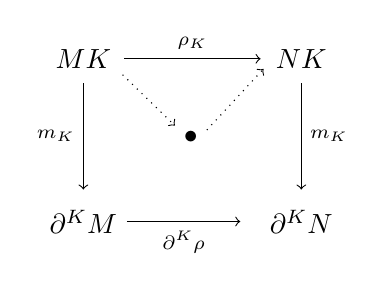
\begin{tikzpicture}[x=1.05em,y=1.05em]
  \node (tl) at (0,3)    {$MK$};
  \node (tr) at (7.5,3)  {$NK$};
  \node (bl) at (0,-2.6) {$\partial^{K}M$};
  \node (br) at (7.5,-2.6) {$\partial^{K}N$};
  \node (pb) at (3.7,0.3) {$\bullet$};
  \draw[->] (1.4,3) -- node[above]{$\scriptstyle\rho_{K}$} (6.1,3);
  \draw[->] (0,2.15) -- (0,-1.5);
  \node at (-0.95,0.35) {$\scriptstyle m_{K}$};
  \draw[->] (7.5,2.15) -- (7.5,-1.5);
  \node at (8.45,0.35) {$\scriptstyle m_{K}$};
  \draw[->] (1.5,-2.6) -- node[below]{$\scriptstyle\partial^{K}\rho$} (5.4,-2.6);
  \draw[->,dotted] (1.35,2.45) -- (3.15,0.7);
  \draw[->,dotted] (4.25,0.55) -- (6.2,2.65);
  \node at (4.9,-0.5) {$\scriptstyle\lrcorner$};
\end{tikzpicture}}}
\end{rveq}
的映射，在 $K$ 的「匹配方块」（matching square）中是一个\trEpimorphism。
\end{definition}

用 C.5 节的术语来说，逐纤维满的映射恰是那些定义\textbf{Reedy \trEpimorphism}的%
\trNaturalTransformation——即那些相对匹配映射 \eqref{eq:matching-square} 为%
\trEpimorphism{}的\trNaturalTransformation。

\begin{lemma}\label{lem:matching-square-pullback}
设 $\rho\colon M\to N$ 是诸 $\mathcal{J}$-结构之间的一个逐纤维满射（fiberwise
surjection）。那么对每个关系
符号 $\dot{R}$，匹配方块是一个\trPullback：
\begin{center}
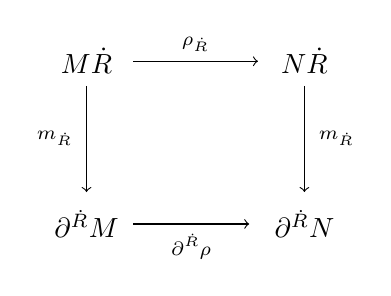
\begin{tikzpicture}[x=1.05em,y=1.05em]
  \node (tl) at (0,3)    {$M\dot{R}$};
  \node (tr) at (7.5,3)  {$N\dot{R}$};
  \node (bl) at (0,-2.6) {$\partial^{\dot{R}}M$};
  \node (br) at (7.5,-2.6) {$\partial^{\dot{R}}N$};
  \draw[->] (1.6,3) -- node[above]{$\scriptstyle\rho_{\dot{R}}$} (5.9,3);
  \draw[->] (0,2.15) -- (0,-1.5);
  \node at (-1.1,0.35) {$\scriptstyle m_{\dot{R}}$};
  \draw[->] (7.5,2.15) -- (7.5,-1.5);
  \node at (8.6,0.35) {$\scriptstyle m_{\dot{R}}$};
  \draw[->] (1.6,-2.6) -- node[below]{$\scriptstyle\partial^{\dot{R}}\rho$} (5.6,-2.6);
  \node at (1.05,2.45) {$\scriptstyle\lrcorner$};
\end{tikzpicture}
\end{center}
\end{lemma}

\begin{proof}
由于 $M$ 与 $N$ 都是 $\mathcal{J}$-结构，$\mathcal{J}$ 的诸关系符号的匹配映射都是%
\trMonomorphism{}（见\cref{ex:folds-matching-map-mono}）。于是，到该\trPullback{}的诱导映射是一个%
\trMonomorphism，而由逐纤维满性假设，它又是一个\trEpimorphism。于是，这个映射
是集合\trCategory{}中的一个\trIsomorphism，故该方块是一个\trPullback。
\end{proof}

请回忆\cref{exa:d-cat-nerve}与\cref{exa:e-d-functors-2cat}中构造的那些结构。

\begin{lemma}\label{lem:surjective-equivalence-fiberwise-surjection}
\begin{enumerate}[label=(\roman*)]
\item \trCategory{}之间的一个\trSurjectiveEquivalence{}
$\mathcal{C}\Rightarrow\mathcal{D}$ 诱导诸 $\mathcal{J}_{\mathcal{C}at}$-结构之间的一个
逐纤维满射 $M_{\mathcal{C}}\Rightarrow M_{\mathcal{D}}$。
\item 2-\trCategory{}之间的一个满射\trBiequivalence{}
$\mathcal{C}\Rightarrow\mathcal{D}$ 诱导诸 $\mathcal{J}_{2\text{-}\mathcal{C}at}$-结构
之间的一个逐纤维满射 $M_{\mathcal{C}}\Rightarrow M_{\mathcal{D}}$。
\end{enumerate}
\end{lemma}

\begin{proof}
这两个陈述是某个更一般的结果的特殊情形，因而有一个公共的证明 [52]。在 $\Cat$ 与
$2\text{-}\Cat$ 上各有一个（余纤维化，平凡纤维化）弱分解系统，其平凡纤维化即陈述中
所指的那些满射双／等价。这些结构是经由应用如下 hom-\trBifunctor{}而定义的
\begin{equation*}
(\Cat^{\mathcal{J}_{\mathcal{C}at}^{\mathrm{op}}})^{\mathrm{op}}\times\Cat
\xrightarrow{\ \mathrm{hom}\ }\Set^{\mathcal{J}_{\mathcal{C}at}}
\qquad\qquad
(2\text{-}\Cat^{\mathcal{J}_{2\text{-}\mathcal{C}at}^{\mathrm{op}}})^{\mathrm{op}}
\times 2\text{-}\Cat
\xrightarrow{\ \mathrm{hom}\ }\Set^{\mathcal{J}_{2\text{-}\mathcal{C}at}}
\end{equation*}
到那些为 Reedy 余纤维性的图表 $D_{\mathcal{C}at}$ 与 $D_{2\text{-}\mathcal{C}at}$ 上。由引理
C.2.11 与推论 C.5.16，相对于由 $\Cat$ 与 $2\text{-}\Cat$ 上的任一弱分解系统以及
$\Set$ 上的（单态射，满态射）弱分解系统所构建的诸 Reedy 弱分解系统，它们都是右
Leibniz 二函子，因为它们是涉及（未富集的）加权余极限二函子的一个双变量伴随中的
右\trAdjunction{}之各项。于是，诸\trFunctor{}
$M_{-}\colon\Cat\to\Set^{\mathcal{J}_{\mathcal{C}at}}$ 与
$M_{-}\colon 2\text{-}\Cat\to\Set^{\mathcal{J}_{2\text{-}\mathcal{C}at}}$ 把平凡纤维化
——即满射双／等价——送到 Reedy \trEpimorphism，即逐纤维满射。
\end{proof}

\begin{definition}\label{def:j-equivalent-in-context}
设 $\mathcal{J}$ 是一个 FOLDS 签名，并设 $\Gamma\colon\mathcal{J}\to\Set$ 是一个带有
给定解释 $\alpha\colon\Gamma\to M$ 与 $\beta\colon\Gamma\to N$ 的上下文，其中
$M,N\colon\mathcal{J}\to\Set$ 为诸 $\mathcal{J}$-结构。诸 $\mathcal{J}$-结构 $M$ 与
$N$ 是\textbf{在上下文 $\Gamma$ 中 $\mathcal{J}$-等价的}（$\mathcal{J}$-equivalent
in context），记作 $M\approx^{\mathcal{J}}_{\Gamma}N$，当且仅当存在一个由 $\Gamma$
之下的诸 $\mathcal{J}$-结构之间的逐纤维满射 $\sigma$ 与 $\rho$ 构成的图表
\begin{center}
\begin{tikzpicture}[x=1.05em,y=1.05em]
  \node (G) at (0,4)   {$\Gamma$};
  \node (M) at (-6,0)  {$M$};
  \node (N) at (6,0)   {$N$};
  \node (P) at (0,-4)  {$P$};
  \draw[->] (-0.95,3.35) -- node[above left,pos=0.45]{$\scriptstyle\alpha$} (-5.2,0.5);
  \draw[->] (0.95,3.35)  -- node[above right,pos=0.45]{$\scriptstyle\beta$} (5.2,0.5);
  \draw[->] (0,3.1)      -- node[right,pos=0.5]{$\scriptstyle\gamma$} (0,-3.1);
  \draw[->] (-0.95,-3.35) -- node[below left,pos=0.55]{$\scriptstyle\sigma$} (-5.2,-0.5);
  \draw[->] (0.95,-3.35)  -- node[below right,pos=0.55]{$\scriptstyle\rho$} (5.2,-0.5);
\end{tikzpicture}
\end{center}
关系「在上下文 $\Gamma$ 中 $\mathcal{J}$-等价」显然是自反的与对称的。事实上，它
也是传递的，读者可在\cref{ex:j-equivalence-transitive}中予以验证。
\end{definition}

\begin{example}\label{exa:jcat-equivalence-iso-comma}
考虑\trCategory{}之间的一个\trEquivalence{} $f\colon\mathcal{C}\to\mathcal{D}$，并经
如下\trPullback{}作出\cref{def:iso-commas}的\trIsoCommaCategory，
\begin{center}
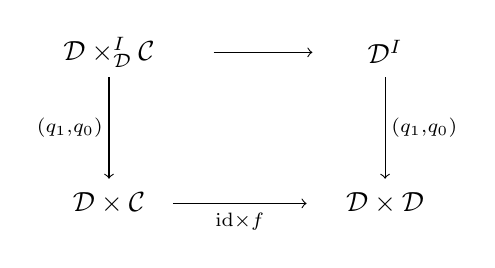
\begin{tikzpicture}[x=1.05em,y=1.05em]
  \node (tl) at (0,2.6)    {$\mathcal{D}\times^{\hciso}_{\mathcal{D}}\mathcal{C}$};
  \node (tr) at (9.5,2.6)  {$\mathcal{D}^{\hciso}$};
  \node (bl) at (0,-2.6)   {$\mathcal{D}\times\mathcal{C}$};
  \node (br) at (9.5,-2.6) {$\mathcal{D}\times\mathcal{D}$};
  \draw[->] (3.6,2.6) -- (7.0,2.6);
  \draw[->] (0,1.75) -- (0,-1.75);
  \node at (-1.35,0) {$\scriptstyle(q_{1},q_{0})$};
  \draw[->] (9.5,1.75) -- (9.5,-1.75);
  \node at (10.85,0) {$\scriptstyle(q_{1},q_{0})$};
  \draw[->] (2.2,-2.6) -- node[below]{$\scriptstyle\mathrm{id}\times f$} (6.8,-2.6);
  \node at (1.05,2.0) {$\scriptstyle\lrcorner$};
\end{tikzpicture}
\end{center}
由于 $f$ 是\trCategory{}之间的一个\trEquivalence，函子
\begin{equation*}
\mathcal{D}\xleftarrow{\ q_{1}\ }
\mathcal{D}\times^{\hciso}_{\mathcal{D}}\mathcal{C}
\xrightarrow{\ q_{0}\ }\mathcal{C}
\end{equation*}
都是\trSurjectiveEquivalence。由\cref{lem:surjective-equivalence-fiberwise-surjection}，%
\cref{exa:d-cat-nerve}的那些朴素 $\mathcal{J}_{\mathcal{C}at}$-结构之间相应的%
\trNaturalTransformation{}是逐纤维满射
\begin{center}
\begin{tikzpicture}[x=1.05em,y=1.05em]
  \node (Mt) at (0,3)   {$M_{\mathcal{D}\times^{\hciso}_{\mathcal{D}}\mathcal{C}}$};
  \node (Ml) at (-6.5,-1) {$M_{\mathcal{C}}$};
  \node (Mr) at (6.5,-1)  {$M_{\mathcal{D}}$};
  \draw[->] (-2.1,2.4) -- node[above left,pos=0.4]{$\scriptstyle q_{0}$} (-5.3,-0.4);
  \draw[->] (2.1,2.4)  -- node[above right,pos=0.4]{$\scriptstyle q_{1}$} (5.3,-0.4);
\end{tikzpicture}
\end{center}
从而在 $M_{\mathcal{C}}$ 与 $M_{\mathcal{D}}$ 之间定义了一个
$\mathcal{J}_{\mathcal{C}at}$-等价。
\end{example}

\begin{example}\label{exa:pseudo-comma-2-category}
考虑 2-\trCategory{}之间的一个\trBiequivalence{} $F\colon\mathcal{C}\to\mathcal{D}$，并
作出\textbf{伪逗号 2-\trCategory}（pseudo-comma 2-category）$\mathcal{P}$，其
\begin{itemize}
\item 对象是三元组 $(x\in\mathcal{C},\,x'\in\mathcal{D},\,a:Fx\simeq x'\in\mathcal{D})$，
  其中 $a$ 是 $\mathcal{D}$ 中的一个\trEquivalence；
\item 1-\trCell{} $(x,x',a)\to(y,y',b)$ 是三元组
\begin{equation*}
\left(
\begin{array}{ccccc}
x & & x' & & Fx\xrightarrow{\ \simeq a\ }x'\\
f\downarrow & \in\mathcal{C}, & f'\downarrow & \in\mathcal{D}, &
Ff\downarrow\ \cong\alpha\ \downarrow f'\ \in\mathcal{D}\\
y & & y' & & Fy\xrightarrow{\ \simeq b\ }y'
\end{array}
\right)
\end{equation*}
\item 2-\trCell{} $(f,f',\alpha)\Rightarrow(g,g',\beta)$ 由一个对
  $(\gamma:f\Rightarrow g\in\mathcal{C},\,\delta:f'\Rightarrow g'\in\mathcal{D})$ 给出，
  使得
\begin{equation*}
\left(
\begin{array}{ccc}
Fx & \xrightarrow{\ \simeq a\ } & x'\\
Ff & \begin{matrix}F\gamma\Downarrow\\ \cong\alpha\end{matrix}\ Fg\ \cong\beta & g'\\
Fy & \xrightarrow{\ \simeq b\ } & y'
\end{array}
\right)
=
\left(
\begin{array}{ccc}
Fx & \xrightarrow{\ \simeq a\ } & x'\\
Ff & \cong\alpha\ \ f'\ \ \delta\Downarrow & g'\\
Fy & \xrightarrow{\ \simeq b\ } & y'
\end{array}
\right)
\end{equation*}
\end{itemize}
显然的投射 $\mathcal{C}\leftarrow\mathcal{P}\to\mathcal{D}$ 定义满射%
\trBiequivalence——即那些于对象上为满、于 1-\trCell{}上为满、且于 2-\trCell{}上为
全忠实的 2-\trFunctor——它们由\cref{lem:surjective-equivalence-fiberwise-surjection}诱导%
\cref{exa:e-d-functors-2cat}的那些饱和 $\mathcal{J}_{2\text{-}\mathcal{C}at}$-结构之间的
逐纤维满的\trNaturalTransformation，从而定义一个 $\mathcal{J}_{2\text{-}\mathcal{C}at}$-等价
\begin{center}
\begin{tikzpicture}[x=1.05em,y=1.05em]
  \node (Mt) at (0,3)    {$M_{\mathcal{P}}$};
  \node (Ml) at (-6.5,-1) {$M_{\mathcal{C}}$};
  \node (Mr) at (6.5,-1)  {$M_{\mathcal{D}}$};
  \draw[->] (-1.9,2.4) -- node[above left,pos=0.4]{$\scriptstyle\sigma$} (-5.1,-0.4);
  \draw[->] (1.9,2.4)  -- node[above right,pos=0.4]{$\scriptstyle\rho$} (5.1,-0.4);
\end{tikzpicture}
\end{center}
\end{example}

这两种构造都可以理解为 Brown 分解 C.1.6 应用于 $\Cat$ 与 $2\text{-}\Cat$ 上的%
\trFolkModelStructure{}中的实例。我们对这些概念的兴趣源于 Makkai 的下述定理：

\begin{theorem}\label{thm:makkai-invariance}
若 $M$ 与 $N$ 在一个上下文 $\Gamma$ 中是 $\mathcal{J}$-等价的
\begin{center}
\begin{tikzpicture}[x=1.05em,y=1.05em]
  \node (G) at (0,4)   {$\Gamma$};
  \node (M) at (-6,0)  {$M$};
  \node (N) at (6,0)   {$N$};
  \node (P) at (0,-4)  {$P$};
  \draw[->] (-0.95,3.35) -- node[above left,pos=0.45]{$\scriptstyle\alpha$} (-5.2,0.5);
  \draw[->] (0.95,3.35)  -- node[above right,pos=0.45]{$\scriptstyle\beta$} (5.2,0.5);
  \draw[->] (0,3.1)      -- node[right,pos=0.5]{$\scriptstyle\gamma$} (0,-3.1);
  \draw[->] (-0.95,-3.35) -- node[below left,pos=0.55]{$\scriptstyle\sigma$} (-5.2,-0.5);
  \draw[->] (0.95,-3.35)  -- node[below right,pos=0.55]{$\scriptstyle\rho$} (5.2,-0.5);
\end{tikzpicture}
\end{center}
那么对所有满足 $\mathrm{var}(\phi)\subset\Gamma$ 的公式 $\phi$，
$M\models\phi[\alpha]$ 当且仅当 $N\models\phi[\beta]$。
\end{theorem}

\begin{proof}
由于 $P$ 本身就是一个 $\mathcal{J}$-结构，并配有由该上下文所定义之变量的一个解释
$\gamma\colon\Gamma\to P$，故只需证明：对任何逐纤维满射 $\sigma\colon P\to M$，$P$
与 $M$ 满足同样的公式：$P\models\phi[\gamma]$ 当且仅当 $M\models\phi[\sigma\gamma]$。
这沿公式 $\phi$ 的复杂度作归纳而得证。

对于基础情形，考虑一个在 $P$ 中带有解释 $x_{p}\mapsto\gamma x_{p}$ 的原子公式
$\dot{R}\langle x_{p}\rangle$。由\cref{lem:matching-square-pullback}的\trPullback，
$\langle\gamma x_{p}\rangle\in\partial^{\dot{R}}P$ 位于 $P\dot{R}$ 中，当且仅当
$\langle\gamma x_{p}\rangle\in\partial^{\dot{R}}M$ 位于 $M\dot{R}$ 中。于是，
$P\models\dot{R}[\gamma]$ 当且仅当 $M\models\dot{R}[\sigma\gamma]$。

接下来考虑由 $\phi$ 与 $\psi$ 构造的复合公式 $\phi\wedge\psi$、$\phi\vee\psi$ 与
$\phi\rightarrow\psi$。在归纳假设下，可以假定 $P\models\phi[\gamma]$ 当且仅当
$M\models\phi[\sigma\gamma]$，对 $\psi$ 亦然。于是立得：$P\models(\phi\wedge\psi)[\gamma]$
当且仅当 $M\models(\phi\wedge\psi)[\sigma\gamma]$，对复合公式 $\phi\vee\psi$ 与
$\phi\rightarrow\psi$ 亦然。

最后，考虑形如 $\forall x\,\phi$ 的公式，其中 $x:K\langle x_{p}\rangle$。解释
$\gamma\colon\mathrm{var}(\forall x\,\phi)\to P$ 在匹配对象中定义了一个元素
$\langle\gamma x_{p}\rangle\in\partial^{K}P$。逐纤维满性条件告诉我们：下右所示的
$K$ 的匹配方块中从 $PK$ 到该\trPullback{}的映射是一个满射：
\begin{center}
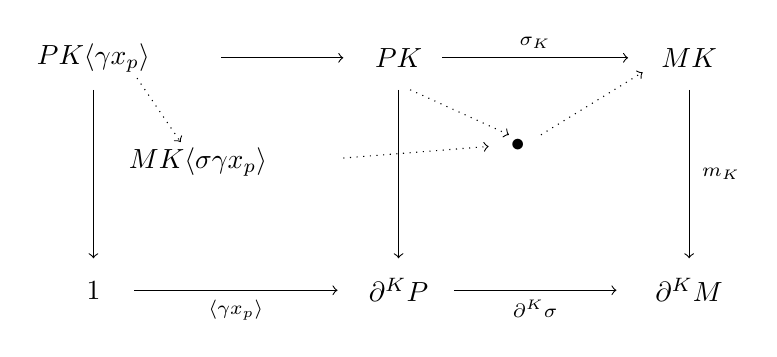
\begin{tikzpicture}[x=1.05em,y=1.05em]
  \node (PKX) at (0,4)     {$PK\langle\gamma x_{p}\rangle$};
  \node (PK)  at (10.5,4)  {$PK$};
  \node (MK)  at (20.5,4)  {$MK$};
  \node (MKX) at (3.6,0.4) {$MK\langle\sigma\gamma x_{p}\rangle$};
  \node (dot) at (14.6,1.0) {$\bullet$};
  \node (one) at (0,-4)    {$1$};
  \node (dKP) at (10.5,-4) {$\partial^{K}P$};
  \node (dKM) at (20.5,-4) {$\partial^{K}M$};
  \draw[->] (4.4,4) -- (8.6,4);
  \draw[->] (12.0,4) -- node[above]{$\scriptstyle\sigma_{K}$} (18.4,4);
  \draw[->] (0,2.9) -- (0,-2.9);
  \draw[->] (10.5,2.9) -- (10.5,-2.9);
  \draw[->] (20.5,2.9) -- (20.5,-2.9);
  \node at (21.6,0) {$\scriptstyle m_{K}$};
  \draw[->] (1.4,-4) -- node[below]{$\scriptstyle\langle\gamma x_{p}\rangle$} (8.4,-4);
  \draw[->] (12.4,-4) -- node[below]{$\scriptstyle\partial^{K}\sigma$} (18.0,-4);
  \draw[->,dotted] (1.5,3.3) -- (3.0,1.1);
  \draw[->,dotted] (8.6,0.55) -- (13.6,0.95);
  \draw[->,dotted] (15.4,1.35) -- (18.9,3.5);
  \draw[->,dotted] (10.9,2.9) -- (14.3,1.35);
  \node at (4.0,4.3) {$\scriptstyle\lrcorner$};
  \node at (8.3,-0.2) {$\scriptstyle\lrcorner$};
  \node at (14.9,0.1) {$\scriptstyle\lrcorner$};
\end{tikzpicture}
\end{center}
通过对\trPullback{}作复合，即得：从 $PK\to\partial^{K}P$ 在 $\langle\gamma x_{p}\rangle$
之上的\trFiber{}到 $MK\to\partial^{K}M$ 在 $\langle\sigma\gamma x_{p}\rangle$ 之上的%
\trFiber{}有一个满射。特别地，若对 $PK\to\partial^{K}P$ 的\trFiber{}中所有 $a$ 都有
$P\models\phi(a/x)[\gamma]$，则由归纳假设 $M\models\phi(\sigma a/x)[\sigma\gamma]$。
由逐纤维满性，$MK\to\partial^{K}M$ 的\trFiber{}中每个元素 $b$ 都等于 $PK\to\partial^{K}P$
的\trFiber{}中某个 $a$ 在 $\sigma$ 下的像，故这告诉我们 $P\models(\forall x\,\phi)[\gamma]$
当且仅当 $M\models(\forall x\,\phi)[\sigma\gamma]$。

类似地，对 $\exists x\,\phi$ 而言，$P\models(\exists x\,\phi)[\gamma]$ 当且仅当在%
\trFiber{}中存在某个 $a$ 使得 $P\models\phi(a/x)[\gamma]$。而这成立当且仅当
$M\models\phi(\sigma a/x)[\sigma\gamma]$，并且由 $\sigma$ 的自然性，$\sigma a$ 居于
恰当的\trFiber{}之中。所以，若 $P\models(\exists x\,\phi)[\gamma]$，则
$M\models(\exists x\,\phi)[\sigma\gamma]$。反之，若 $M\models(\exists x\,\phi)[\sigma\gamma]$，
则在 $MK\to\partial^{K}M$ 于 $\langle\sigma\gamma x_{p}\rangle$ 之上的\trFiber{}中有
某个 $b$ 使得 $M\models\phi(b/x)[\sigma\gamma]$。由逐纤维满性，在 $PK\to\partial^{K}P$
于 $\langle\gamma x_{p}\rangle$ 之上的\trFiber{}中有某个 $a$ 使得 $\sigma a=b$。由归纳
假设，$P\models\phi(a/x)[\gamma]$ 当且仅当 $M\models\phi(b/x)[\sigma\gamma]$，故我们
看到：若 $M\models(\exists x\,\phi)[\sigma\gamma]$，则 $P\models(\exists x\,\phi)[\gamma]$。
\end{proof}

\begin{remark}\label{rem:henry-observation}
Henry 的一个观察 [52] 为 Makkai 的\cref{thm:makkai-invariance}提供了一个不错的
视角。Henry 证明：对一个取定的 FOLDS 签名 $\mathcal{J}$，诸公式的搜集定义了从该
签名的上下文\trCategory{}到布尔代数的始函子，并带有如下性质：与显示映射相关联的
限制\trHomomorphism{}容有左、右\trAdjunction{}（即存在量化与全称量化），且满足 Beck--Chevalley
条件。通过取幂集，任何 $\mathcal{J}$-结构都给出一个从上下文\trCategory{}到布尔代数
的典范\trFunctor，而来自始对象的唯一映射把一个公式送到由其自由变量的、满足该公式
的那些解释构成的子集。诸 $\mathcal{J}$-结构之间的一个映射 $\rho$ 在相应的布尔代数
值\trFunctor{}之间定义了一个\trNaturalTransformation——经由重指标化，这是反变的
——并且这一\trNaturalTransformation{}保持左、右伴随，当且仅当 $\rho$ 是逐纤维满的。
于是，由始性我们便看到：逐纤维满射保持公式的解释。
\end{remark}

\subsection*{练习}

\begin{exercise}\label{ex:folds-matching-map-mono}
设 $\mathcal{J}$ 是一个带有关系符号 $\dot{R}\in\mathcal{J}$ 的 FOLDS 签名，并设
$M\colon\mathcal{J}\to\Set$ 是任何\trFunctor。证明：\cref{def:j-structure}的映射是一个%
\trMonomorphism{}当且仅当观察 C.1.18 的匹配映射是一个\trMonomorphism：
\begin{center}
\begin{tikzpicture}[x=1.05em,y=1.05em]
  \node (MR)   at (0,0.9)  {$M\dot{R}$};
  \node (prod) at (10.5,0.9)
    {$\displaystyle\prod_{p\colon \dot{R}\to^{\neq}K_{p}} MK_{p}$};
  \node (lim)  at (4.8,-1.5)
    {$\partial^{\dot{R}}M\coloneqq\displaystyle\lim_{p\colon \dot{R}\to^{\neq}K_{p}} MK_{p}$};
  \draw[->] (1.5,0.9) -- (7.2,0.9);
  \draw[->,dashed] (0.5,0.3) -- (3.4,-0.85);
  \node at (1.0,-0.65) {$\scriptstyle m^{\dot{R}}$};
  \draw[right hook->] (7.7,-1.05) -- (9.8,0.3);
\end{tikzpicture}
\end{center}
\end{exercise}

\begin{exercise}\label{ex:var-subcontext}
\begin{enumerate}[label=(\roman*)]
\item 证明：若 $\phi$ 是任何公式，则 $\mathrm{var}(\phi)$ 对依赖封闭：若
  $x\in\mathrm{var}(\phi)$，则 $\mathrm{dep}(x)\subset\mathrm{var}(\phi)$。
\item 证明：在上下文 $\Gamma$ 中为具体公式 $\phi$ 定义的诸变量 $\mathrm{var}(\phi)$
  定义一个子上下文 $\mathrm{var}(\phi)\subset\Gamma$。
\end{enumerate}
\end{exercise}

\begin{exercise}\label{ex:biterminal-sentence}
2-\trCategory{} $\mathcal{C}$ 中的一个对象 $s$ 是\textbf{双终的}（biterminal），若对
每个 $c\in\mathcal{C}$，hom-\trCategory{} $\mathcal{C}(c,s)\simeq 1$ 是一个%
\trContractible{}\trGroupoid。请写出一个 2-\trCategory{}语言中的语句，断言该
2-\trCategory{}有一个双终对象。
\end{exercise}

\begin{exercise}\label{ex:matching-square-statement}
请把\cref{lem:matching-square-pullback}的结果与如下陈述联系起来：对某个解释
$\alpha\colon\Gamma\to M$，$M\models\dot{R}[\alpha]$ 当且仅当 $N\models\dot{R}[\rho\alpha]$。
\end{exercise}

\begin{exercise}\label{ex:j-equivalence-transitive}
请通过复合由逐纤维满射构成的那些\trSpan{}来验证\cref{def:j-equivalent-in-context}所
定义的关系是传递的。
\end{exercise}

\begin{exercise}\label{ex:naive-not-j-equivalent}
请沿用\cref{exa:equivalence-sentence-j2cat}中所考虑的那一类语句或公式，并利用%
\cref{thm:makkai-invariance}的结果证明：存在双等价的 2-\trCategory{} $\mathcal{C}$
与 $\mathcal{D}$，使得在某个适当的上下文中，朴素 $\mathcal{J}_{2\text{-}\mathcal{C}at}$-结构
$N_{\mathcal{C}}$ 与 $N_{\mathcal{D}}$ 并非 $\mathcal{J}_{2\text{-}\mathcal{C}at}$-等价的。
\end{exercise}









